% Chapter 1

\chapter[Motivation and Background]
{Motivation and Background} % Main chapter title

\label{Chapter1} % For referencing the chapter elsewhere, use \ref{Chapter1} 

%----------------------------------------------------------------------------------------

% Define some commands to keep the formatting separated from the content 
\newcommand{\keyword}[1]{\textbf{#1}}
\newcommand{\tabhead}[1]{\textbf{#1}}
\newcommand{\code}[1]{\texttt{#1}}
\newcommand{\file}[1]{\texttt{\bfseries#1}}
\newcommand{\option}[1]{\texttt{\itshape#1}}

%----------------------------------------------------------------------------------------

\section[Quantum info processing and Qubit candidates]{Quantum info processing and Qubit candidates}


%----------------------------------------------------------------------------------------

\section[Silicon vacancy as a Qubit candidate]{Silicon vacancy as a Qubit candidate}
\begin{figure}[h]
\centering
\includegraphics[width=0.7\linewidth]{../pic/WP_20160921_20_40_25_Pro_LI}
\caption{}
\label{fig:wp20160921204025proli}
\end{figure}
\begin{figure}[h]
\centering
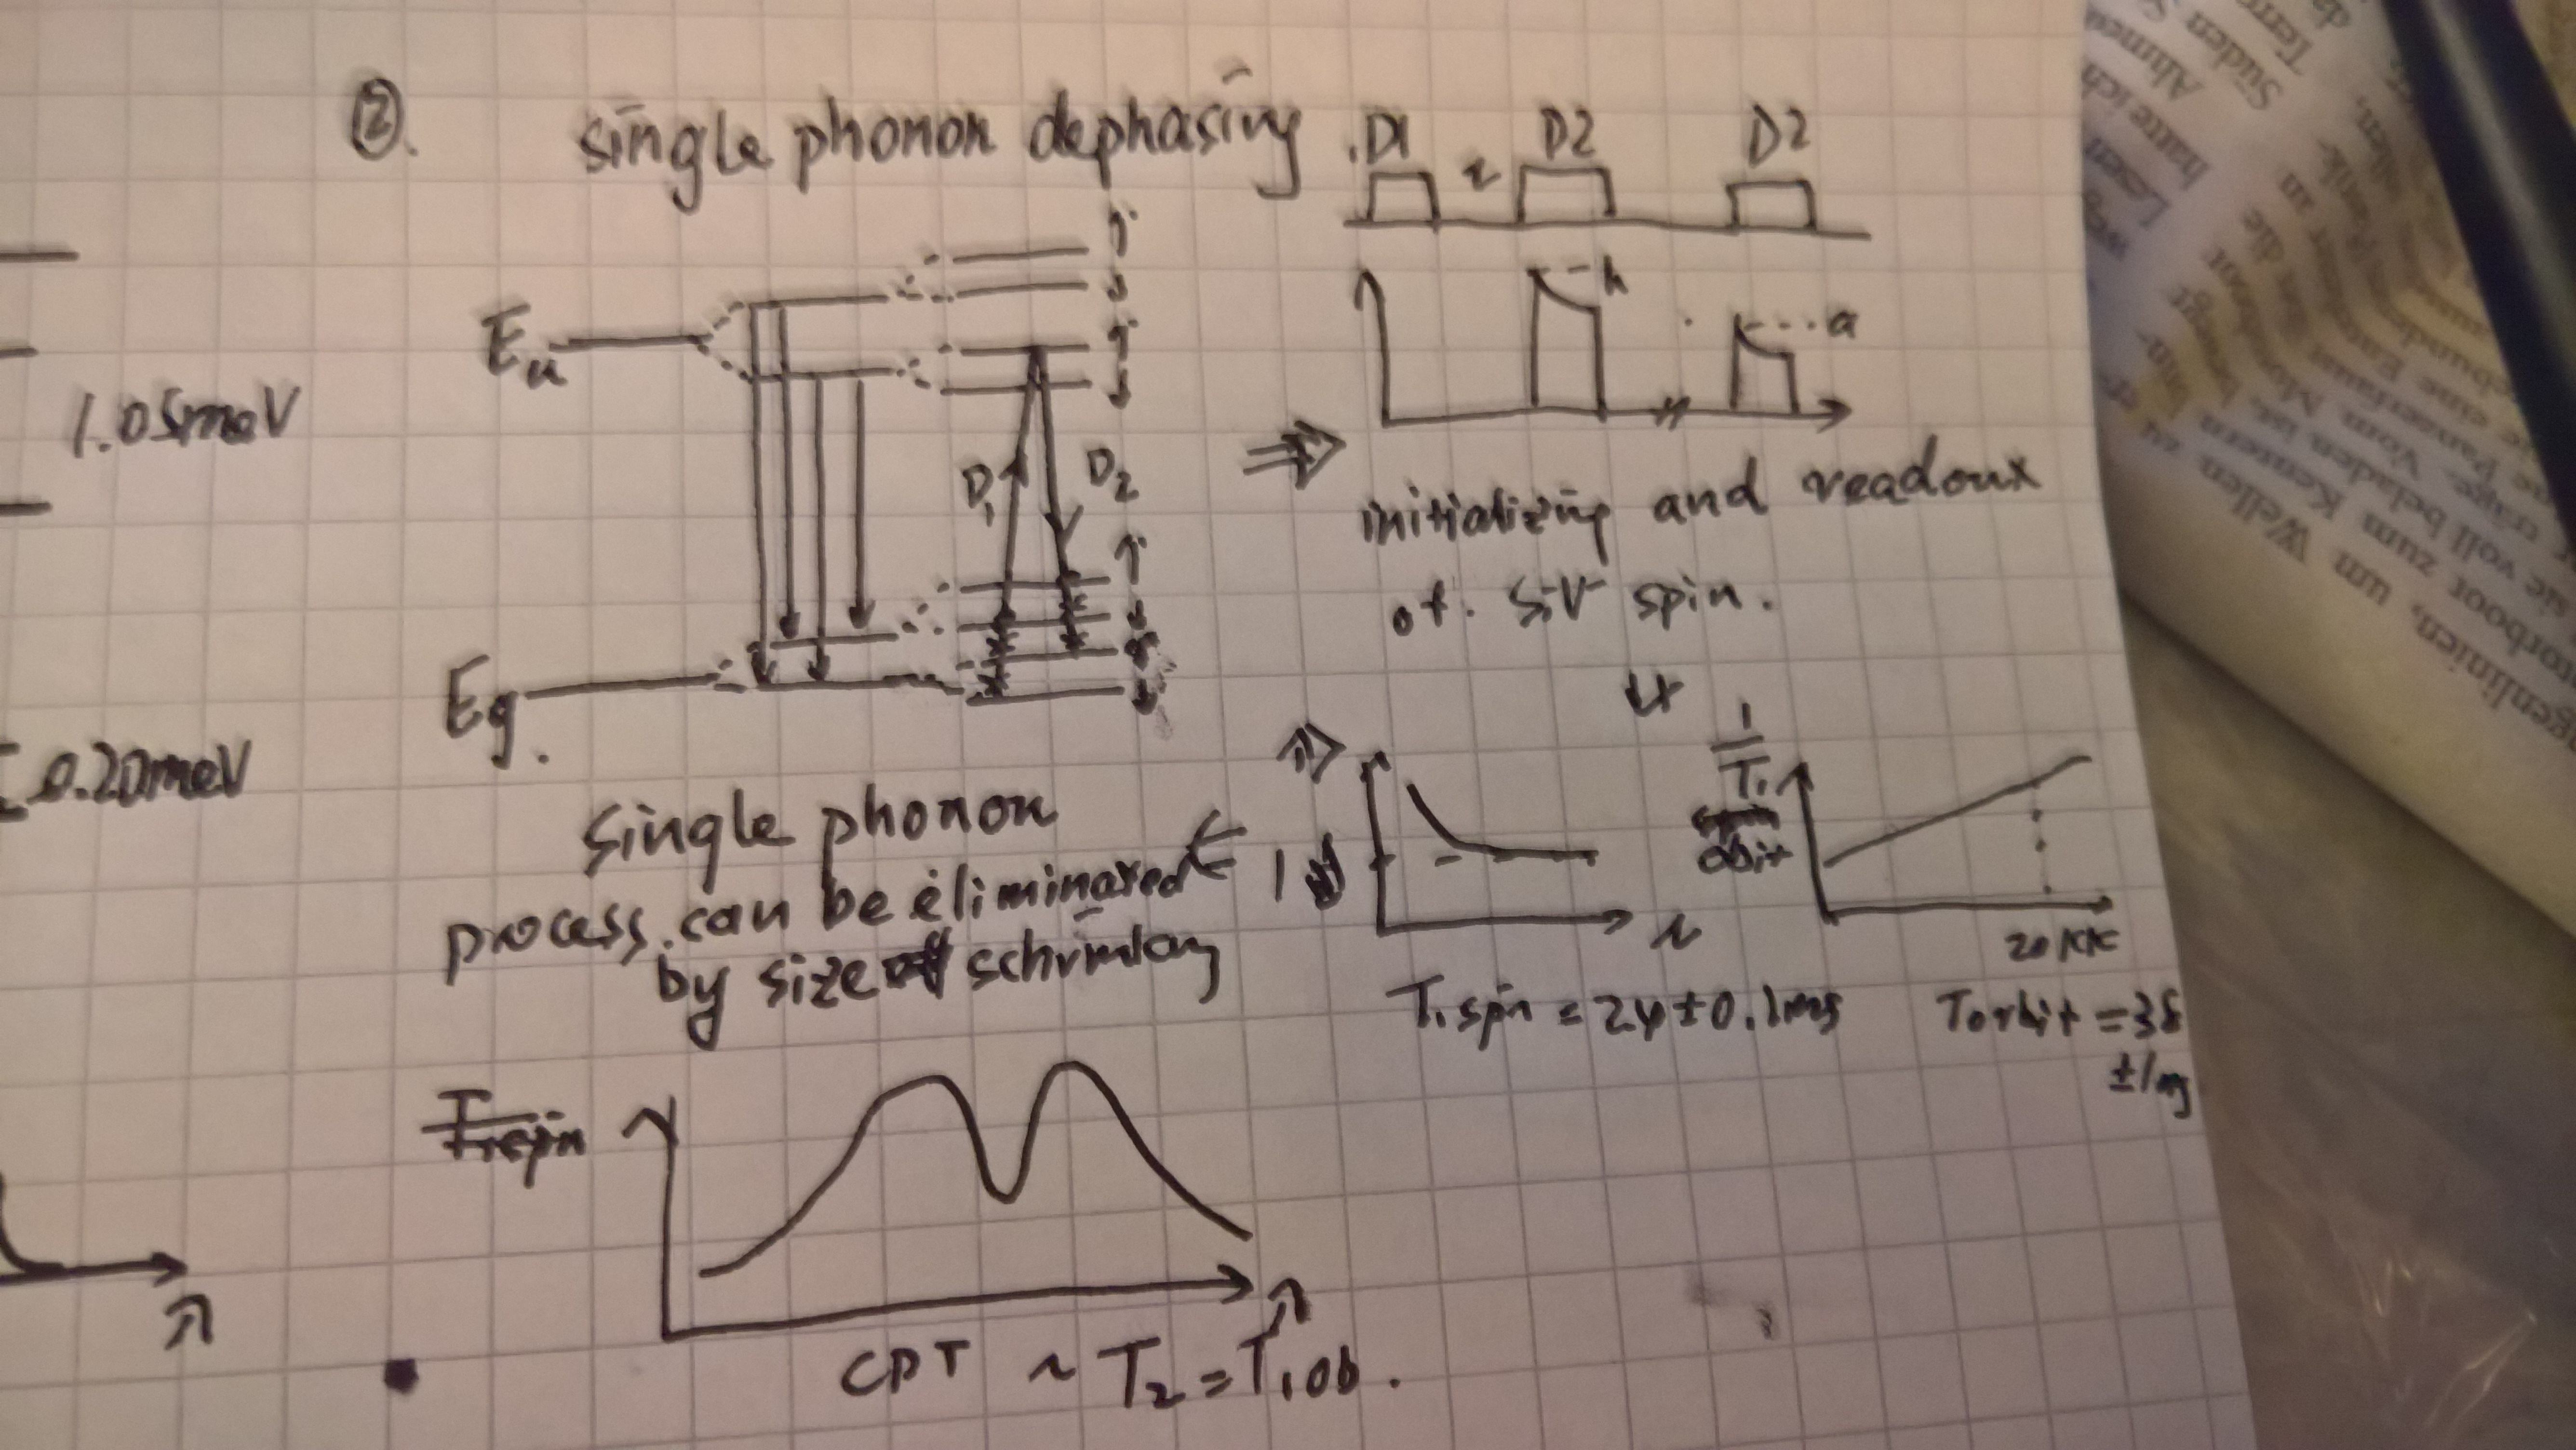
\includegraphics[width=0.7\linewidth]{../pic/WP_20160921_20_40_32_Pro_LI}
\caption{}
\label{fig:wp20160921204032proli}
\end{figure}

%----------------------------------------------------------------------------------------

\section[Silicon vacancies in nanodiamonds]{Silicon vacancies in nanodiamonds}
\begin{figure}[h]
\centering
\includegraphics[width=0.7\linewidth]{../pic/WP_20160921_20_40_48_Pro_LI}
\caption{}
\label{fig:wp20160921204048proli}
\end{figure}
\begin{figure}[h]
\centering
\includegraphics[width=0.7\linewidth]{../pic/WP_20160921_20_40_42_Pro_LI}
\caption{}
\label{fig:wp20160921204042proli}
\end{figure}


SiV in NDs typically worse optical properties.

We already have some of the best SiV in NDs ever seen [Uwe's paper].

However, even these show clear spectral diffusion at the PL spectrometer resolution.

These are not good enough to perform the desired orbital T1 adn then spin T2 measurements.

%----------------------------------------------------------------------------------------

\section[Motivation of the thesis, unsolved problem]{Motivation of the thesis, unsolved problem}
Improve optical properties, 
\paragraph{methods of surface termination}
